\documentclass[reprint]{revtex4-2}
\usepackage{graphicx}
\usepackage{amsmath}
\usepackage{amssymb}
\usepackage{physics}
\usepackage{hyperref}

\newtheorem{definition}{Definition}
\newtheorem{proposition}{Proposition}
\newtheorem{theorem}{Theorem}
\newtheorem{lemma}{Lemma}
\newtheorem{corollary}{Corollary}
\bibliographystyle{plain}

\DeclareMathOperator*{\argmax}{argmax}
\DeclareMathOperator*{\argmin}{argmin}
\newcommand{\sym}[1]{\text{Sym}\qty[#1]}
\newcommand{\asym}[1]{\text{Asym}\qty[#1]}


\begin{document}
\title{Partial Dual Method for Solving QCQPs}
\author{Justin Cardona}
\affiliation{Engineering Physics Department, Polytechnique Montréal}
\begin{abstract}
This work implements a computationally inexpensive method to solve indefinite quadratically constrained quadratic programs (QCQPs). Using the Lagrange dual perspective, the need to use a barrier method to check for dual feasibility is circumvented using a \textit{Partial Dual} that leverages one of the positive definite constraints. This method trades the tens of thousands of matrix-vector products needed in trace estimation solutions for order 10 inverse solves.
\end{abstract}
\maketitle


\section{Introduction}
\label{sec:introduction}

Inverse design in photonics relies heavily on being able to investigate large numbers of unintuitive geometries. However, because the design parameter space is typically extremely large local methods are typically employed. As such the designs created by current programs provide little certainty on providing globally optimal results. There have been recent efforts to to establish bounds on the performance of these methods by using Lagrange duality. However, currently available optimization methods do not allow for computationally efficient means to perform the dual optimization\cite{molesky2020global}. This typically involves doing positive-definite checks using eigenvalue decomposition, which is not practical for extremely large systems. There is a promising method \cite{molesky2020hierarchical} that employs a \textit{Partial Dual} perspective to alleviate some of the complexity. This approach considers another dual program to the primal by leveraging one of its positive definite constraints to avoid the need to do positive definite checks on the program as a whole. However, for large system sizes current methods for forming this problem are still infeasible. Thus the focus of this paper is to present a computationally inexpensive algorithm that can implement the partial dual perspective. The general idea is to use Padé approximants to fit to a positive definite constraint function using very few sample points. While generating the sample points is computationally expensive, working with the approximation is cheap. In section \ref{sec:background} the optimization problem is introduced along with an overview of why current methods are not computationally pratical. In section \ref{sec:algorithm}, the workaround to this problem is presented.

\section{Background}
\label{sec:background}

In this work a numerical scheme is considered for performing inverse design. Firstly the volume where the device must lie is discretized (into a cartesian grid for example). A field in this perspective is represented by a vector with entries that correspond to the polarization current of each cell. For example, if a volume is divided into an $n\times n\times n$ grid then a polarization current can be represented using a vector in $\mathbb{C}^{3n^3}$. Additionally, they can be considered vectors in a Hilbert space with the following inner product:

\begin{align}
	\braket{F}{G} = \int_{\mathbb{R}^3} \dd[3]{x} F^*(x)\cdot G(x)
	\label{eq:inner-product}
\end{align}
Strictly speaking, the Hilbert space being discussed has the above product where the vectors are all elements of $\mathbb{C}^{3n^3}$ that correspond to a physical current/field. In any case, discussing this directly is not particularly important for the rest of this discussion. What is important however, is that physical fields respect the symmetry, linearity, and positive definiteness requirements of a Hilbert space. This can be quickly verified using equation \ref{eq:inner-product}.

\subsection{Problem Formulation}
\label{ssec:formulation}
With this in mind, consider the following quadratic program:

\begin{align}
	\max_{\ket{T}\in\mathbb{C}^{3n^3}} \Im\braket{S}{T} - \ev{O}{T}
\end{align}
In general, $\ket{S}$ can be any element in $\mathbb{C}^{3n^3}$ and $O$ is some general objective linear operator on the space. In the case of Purcell enhancement for example, $O=\asym{V^{-\dagger}}$ is an appropriate choice. Without loss of generality, it is convenient in the photonics context to have it represent the source field of the problem (which must be scattered to acheive the desired objective) explicitly. Given a source field $\ket{S}$ and a scattering potential $V$, the total field $\ket{T}$ produced is given by

\begin{align}
	\ket{T} = \qty(V^{-1} - G_0)^{-1}\ket{S},
\end{align}
where $G_0$ is the Green's function of Maxwell's equations for free space. To this objective function constraints are added to enforce power conservation using a hierarchical mean field approach\cite{molesky2020hierarchical}. This is done by considering connected clusters ($\vb{\Omega} = \qty{\Omega_k}_{k\in K}$) within the design domain and imposing constraints in one of the following forms $\forall \Omega_k\in\vb{\Omega}$:

\begin{align}
	\mel{S}{\mathbb{I}_{\Omega_k}}{T} &= \mel{T}{U\mathbb{I}_{\Omega_k}}{T}\\
	\mel{S}{\mathbb{I}_{\Omega_k}}{R} &= \mel{R}{\mathbb{I}_{\Omega_k}}{R}\notag\\
	\mel{S}{\mathbb{I}_{\Omega_k}}{T} &= \mel{R}{\mathbb{I}_{\Omega_k}}{T}\notag\\
	\mel{S}{\mathbb{I}_{\Omega_k}}{R} &= \mel{T}{U\mathbb{I}_{\Omega_k}}{R}\notag
\end{align}
Here $\mathbb{I}$ is an indicator function over its subscript and $U=V^{-\dagger}-G_o^\dagger$. In order to obtain bounds on this program P, the Lagrange dual program D(P) is considered, the corresponding Lagrangian is

\begin{align}
	\mathcal{L} = \mqty[\bra{T} & \bra{S}]\mqty[-Z^{TT} & Z^{TS} \\ Z^{ST} & 0]\mqty[\ket{T} \\ \ket{S}]
\end{align}
where

\begin{align}
	\label{eq:lagrange_vars}
	Z^{TT} &= O + \sym{U\Phi_1} + \asym{U\Phi_2}\\
	Z^{TS} = Z^{ST*} &= \frac{1}{2}\qty(\Phi_1 + i\Phi_2)I.\notag
\end{align}
In this notation $\Phi_1 \in \mathbb{R}_{\ge 0}^{n_1}$ and $\Phi_2 \in \mathbb{R}_{\ge 0}^{n_2}$ contain the Lagrange multipliers associated with the $n_1$ symmetric and $n_2$ antisymmetric cluster constraints. The dual function is then $\mathcal{G} = \max_{\ket{T}}\mathcal{L}\qty(\ket{T}, \Phi)$ for the dual program:

\begin{align}
	\text{D}\qty(P) = \inf_{\Phi} \mathcal{G}(\Phi)
\end{align}
This problem is typically solved using local methods (newton-like gradient descents for example). 

\subsection{Issues with Standard Dual Solutions}
\label{ssec:formulation}
A notable feature of this problem is that $Z^{TT}$ is indefinite in general, so it may not have a global extremum and diverge in certain regions. In order to obtain a bound on the primal, these regions must be avoided so it must be verfied whether $Z^{TT}\succcurlyeq 0$ for each value of $\Phi$ tested. To do this explicitly requires finding the eigenvalues of the matrix, typically done with a Cholesky-like decoposition. The discretizations typically require $n$ in the hundreds, make doing this check at each point in the optimization far to costly.\\

A common attempt to remedy this is to use the $\log\det Z^{TT}$ in order to ascertain when the boundary of the positive-definiteness is nearby. Assuming that $Z^{TT}$ is positive definite to begin with, when a value of $\Phi$ is chosen such that $Z^{TT}$ is close to being indefinite there will be eigenvalues that start to approach zero. Since the determinant is the product of the eigenvalues, it is naively expected that it also become very small. Therefore, the $\log\det$ is expected to become very large around the the boundary. The reason that this method is advantageous over eigenvalue solvers is that a Hutchinson trace estimator can be used ($\log\det Z^{TT} = \Tr\log Z^{TT}$). Briefly, for any square matrix $A\in\mathbb{C}^{m\times m}$ the Hutchinson trace estimator does probabilistic sampling over vector-matrix-vector products to estimate the trace:

\begin{align}
	\Tr_A\approx\frac{1}{N}\sum_{i=1}^N x^\dagger Ax,\ x\sim\qty{-1, 1}^m
\end{align}
This method, however is still too slow. In order to obtain relative error $\epsilon$ to probability $1-\delta$ the number of sample vectors needed is \cite{skorski2021modern}

\begin{align}
	N = \frac{2}{\epsilon^2}\qty(2+\frac{8\sqrt{2}}{3}\epsilon)\log\frac{2}{\delta}.
\end{align}
For reference a 99.9\% chance to have 0.1\% error needs 30 460 939 matrix vector products, and a 75\% chance to have 1\% error needs 84 746 matrix vector products.
\section{Padé Algorithm}
\label{sec:algorithm}
In order to avoid this expensive step another method must be employed to guarantee the points tested are within the positive definite domain. Therefore a modification of the dual function is considered (the \emph{Partial Dual} $\text{D}_\partial(\text{P})$), singling out one of the constraints,

\begin{align}
	&\mathcal{G}_\partial = \max_{\ket{T}}\mathcal{L}_\partial\qty(\ket{T}, \Phi)\\
	\text{such that } &\Im\braket{S}{T} - \ev{E}{T}\ge 0 \notag
\end{align}
such that

\begin{align}
	\mathcal{L}_\partial = \mqty[\bra{T} & \bra{S}]\mqty[-Z^{TT}_\partial & Z^{TS}_\partial \\ Z^{ST}_\partial & 0]\mqty[\ket{T} \\ \ket{S}].
\end{align}
Here the $\partial$ subscript for the partial dual problem denotes that the quantity is the same as in the ordinary case, except for the fact that terms containing the dual constraint have been removed. If $Z^{T}_\partial\succcurlyeq 0$ then the problem is convex and no checking is required. In this case, $\text{D}_\partial(\text{P}) = \ev{Z^{TS}_\partial Z^{TT-1}_\partial Z^{TS}_\partial}{S}$ with the corresponding current $\ket{\vb{T}} = Z^{TT-1}_\partial Z^{TS}_\partial\ket{S}$.\\

Therefore, the idea of this method is that a feasible $\zeta$ (the dual constraint's multiplier) must be chosen such that $Z^{TT}_\partial$ is positive definite. Note that $Z^{TT}_\partial = Z^{TT} + \zeta E$ and $Z^{TS}_\partial = Z^{TS} + \frac{1}{2}i\zeta I$ so the constraint function is implicitly dependant on $\zeta$, so it will hereafter be abbreviated to $C_\zeta$. With this notation, the goal is to have $\zeta$ such that

\begin{align}
	Z^{TT}+\zeta E&\succcurlyeq0\\
	C_\zeta&\ge0 \notag
\end{align}
Since $E\succcurlyeq0$, $\exists\zeta\ge0$ such that $Z^{TT}_\partial\succcurlyeq0$. Next note that the derivative of the constraint areas follows:

\begin{align*}
	\frac{dC_\zeta}{d\zeta} &= 2\qty(\frac{1}{2}\bra{S} - i\bra{T}E)Z^{TT-1}_\partial\qty(\frac{1}{2}\ket{S}+ iE\ket{T})\\
	\frac{d^2C_\zeta}{d\zeta} &= -6\qty(\frac{1}{2}\bra{S} - i\bra{T}E)Z^{TT-1}_\partial E Z^{TT-1}_\partial\qty(\frac{1}{2}\ket{S}+ iE\ket{T})
\end{align*}
Therefore if $Z^{TT}_\partial\succcurlyeq0$, then $C_\zeta$ must be increasing and concave. Furthermore, in the limit of large $\zeta$:

\begin{align}
	&\lim_{\zeta\rightarrow\infty}Z^{TT-1}_\partial = \qty(\zeta E)^{-1}\\
	&\lim_{\zeta\rightarrow\infty}Z^{TS}_\partial = \frac{1}{2}i\zeta I \notag\\
	\implies&\lim_{\zeta\rightarrow\infty} C_\zeta = \ev{E^{-1}}{S}\notag
\end{align}
Since $E\succcurlyeq0$, $C_\zeta$ asymptotes to a positive number. The combination of these properties of the constraint mean that if a zeta is chosen past the last crossing, it is feasible and makes the problem convex.

The next logical step is to find an efficient way to find the last zero of this constraint function. The issue is that evaluating $C_\zeta$ is very expensive to evaluate since it involves doing an inverse solve for a very large system, so it must be done sparingly. For this reason, the strategy here is to create a series approximation of $C_\zeta$. The last root of the series ought to be computationally cheap to find and should be able to capture the beviour of poles, of which the constraint function has many. Therefore, a Padé approximant is well suited for the task.

\subsection{The AAA Algorithm}
The Padé approximant is constructed according to the AAA algorithm \cite{nakatsukasa2018aaa}, this is done as follows: Consider a function $f:\mathbb{C}\rightarrow\mathbb{C}$, the goal is to find another function $r:\mathbb{C}\rightarrow\mathbb{C}$ to approximate it. Given a finite ordered set $Z\subset\mathbb{C}$ and its corresponding $f$ values $F\subset\mathbb{C}$. The AAA algorithm will split $Z$ and $F$, each into 2 partitions. The first partitions ($z^m$ and $f^m$) will be used to make the $m$ support point in the Padé series:

\begin{align}
    r(z) = \frac{n(z)}{d(z)}=\sum_{j=1}^m\frac{w_jf_j}{z-z_j}\left/ \sum_{j=1}^m\frac{w_j}{z-z_j}\right.
\end{align}
The second partitions ($Z^m = Z\setminus z^m$ and $F^m = F\setminus f^m$) will be used as sample points to do a least squares fit the series, thus determining the weights. This is accomplished in the following way:
\begin{enumerate}
    \item $f^1 = \qty{\argmin_{f\in F}(f-\ev{F})^2}$ and $z^1$ is the corresponding singleton. This defines $F^1$ and $Z^1$.
    \item Obtain $w^1$ by performing a least squares fit to $F^1$ and $Z^1$ using $f^1$ and $z^1$ as the support point.
    \item Given $F^m$, $Z^m$, $f^m$, $z^m$, and $w^m$ calculate the square residuals for all $z\in Z^m$. Select the $(z, f)\in Z^m\times F^m$ with the least residual and add it to the support points.
    \item Using the newly obtained $f^{m+1}$ and $z^{m+1}$, obtain $w^{m+1}$ by least squares fitting to $F^{m+1}$ and $Z^{m+1}$.
    \item Repeat steps 3 and 4 until the desired error tolerance is reached.
\end{enumerate}

\subsection{Finding the Last $C_\zeta$ Root}
Now for how this is applied to the partial dual:

\begin{enumerate}
    \item Sample on a uniform distribution centered on an initial guess to form $Z$ and use $C_\zeta$ to form $F$.
    \item Form the AAA approximant of $C_\zeta$ using $Z$ and $F$ and find the zero of the approximant $\zeta_\text{guess}$
    \item If $C_{\zeta_\text{guess}}$ is not within tolerance, add $(\zeta_\text{guess}, C_{\zeta_\text{guess}})$ to $(Z, F)$ and return to step 2.
\end{enumerate}
While finding the initial guess might be costly, this must only be done once in the entire inverse design. In subsequent steps in a search in the Lagrange multiplier space, the $Z$ matrices are perturbed according to their dependance on $\Phi$. Since their dependance is continuous, it is expected that small changes in $\Phi$ will result in small changes in the last zero crossing.

\section{Results}
\label{sec:results}
In order to test the efiiciency of the root finding algorithm, statistical test is done to find the typical behaviour. This is accomplished by randomly sampling the variables that appear in equation \ref{eq:lagrange_vars}. The distributions are uniform over the domains seen in Table \ref{tab:domains}.

\begin{table}[!htp]
\begin{tabular}{|c|c|}
\hline
Variable & Sampling Domain                   \\ \hline
$O$      & $[0, 1]$ \\ \hline
$S$      & $[-0.5, 0.5]\times[-0.5i, 0.5i]$  \\ \hline
$V$      & $[]\times[0, 10^{-3}i]$  \\ \hline
$\Phi$   & [0, 1]                            \\ \hline
\end{tabular}
\caption{Each element of the discretized quantities is sampled from the distribution. The interval notation is taken to represent the line segment in the complex plane bounded by the two points.}
\label{tab:domains}
\end{table}

The root finding method on average takes $4.65\pm 2.89$ inverse solves to terminate.

\begin{figure}[!htp]
	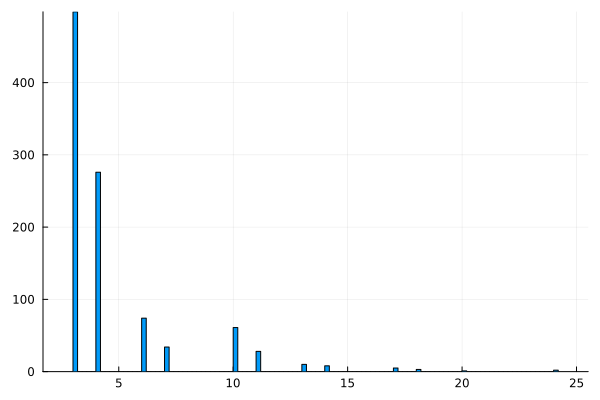
\includegraphics[width=\linewidth]{histogram.png}
	\caption{Histogram of the number of inverse solves it takes for the algorithm to terminate. Note the behaviour where there is a peridodic appearance of peaks, this is due to the fact that the for testing there is a maximum iteration imposed, after which resampling occurs.}
\end{figure}

\bibliography{references}
\end{document}
